\subsection{Tracking}

A charged particle produced in a decay of a heavy flavour meson exiting the \pv is first detected
as \emph{hits} in the \velo.
The \velo subdetector is made up of 21 modules orientated in the \plane{x}{y}, and
each module consists of two layers of silicon strip detectors with $(r,\phi)$ coordinates.
The pitch of the silicon strips vary from \approx$40\mum$ nearest the centre, where detector occupancy
is highest, to \approx$100\mum$ at the extremities.

Spacial resolution is vitally important so close to the interaction point.
The \velo must be able to resolve all tracks and distinguish \pv{s} coming from
proton-proton interactions, and secondary vertices indicative of decaying heavy flavour hadrons.
For example, a \Bp meson with a momentum of $100\gev$ will travel approximately $1\cm$ before decaying.
This must all be done in a high track multiplicity environment.

%Tracking begins with the \velo which precisely measures spatial
%coordinates of charged particle close to the interaction point.

% increase spatial resolution of vertices,
To decrease the distance of extrapolation of tracks to vertices,
the active area of the \velo starts $8\mm$ from the beam line.
This is made possible because each module is split into two halves which retract when the \lhc beam
is unstable.
%Its design leads to a detector with high impact parameter resolution, which can detect tracks
%emerging from a proton-proton interaction in the range $1.6<\eta<4.9$ and $|z|<10.6\cm$.
Figure~\ref{fig:lhcb:velo} shows the geometry of the \velo.

\begin{figure}
  \begin{center}
    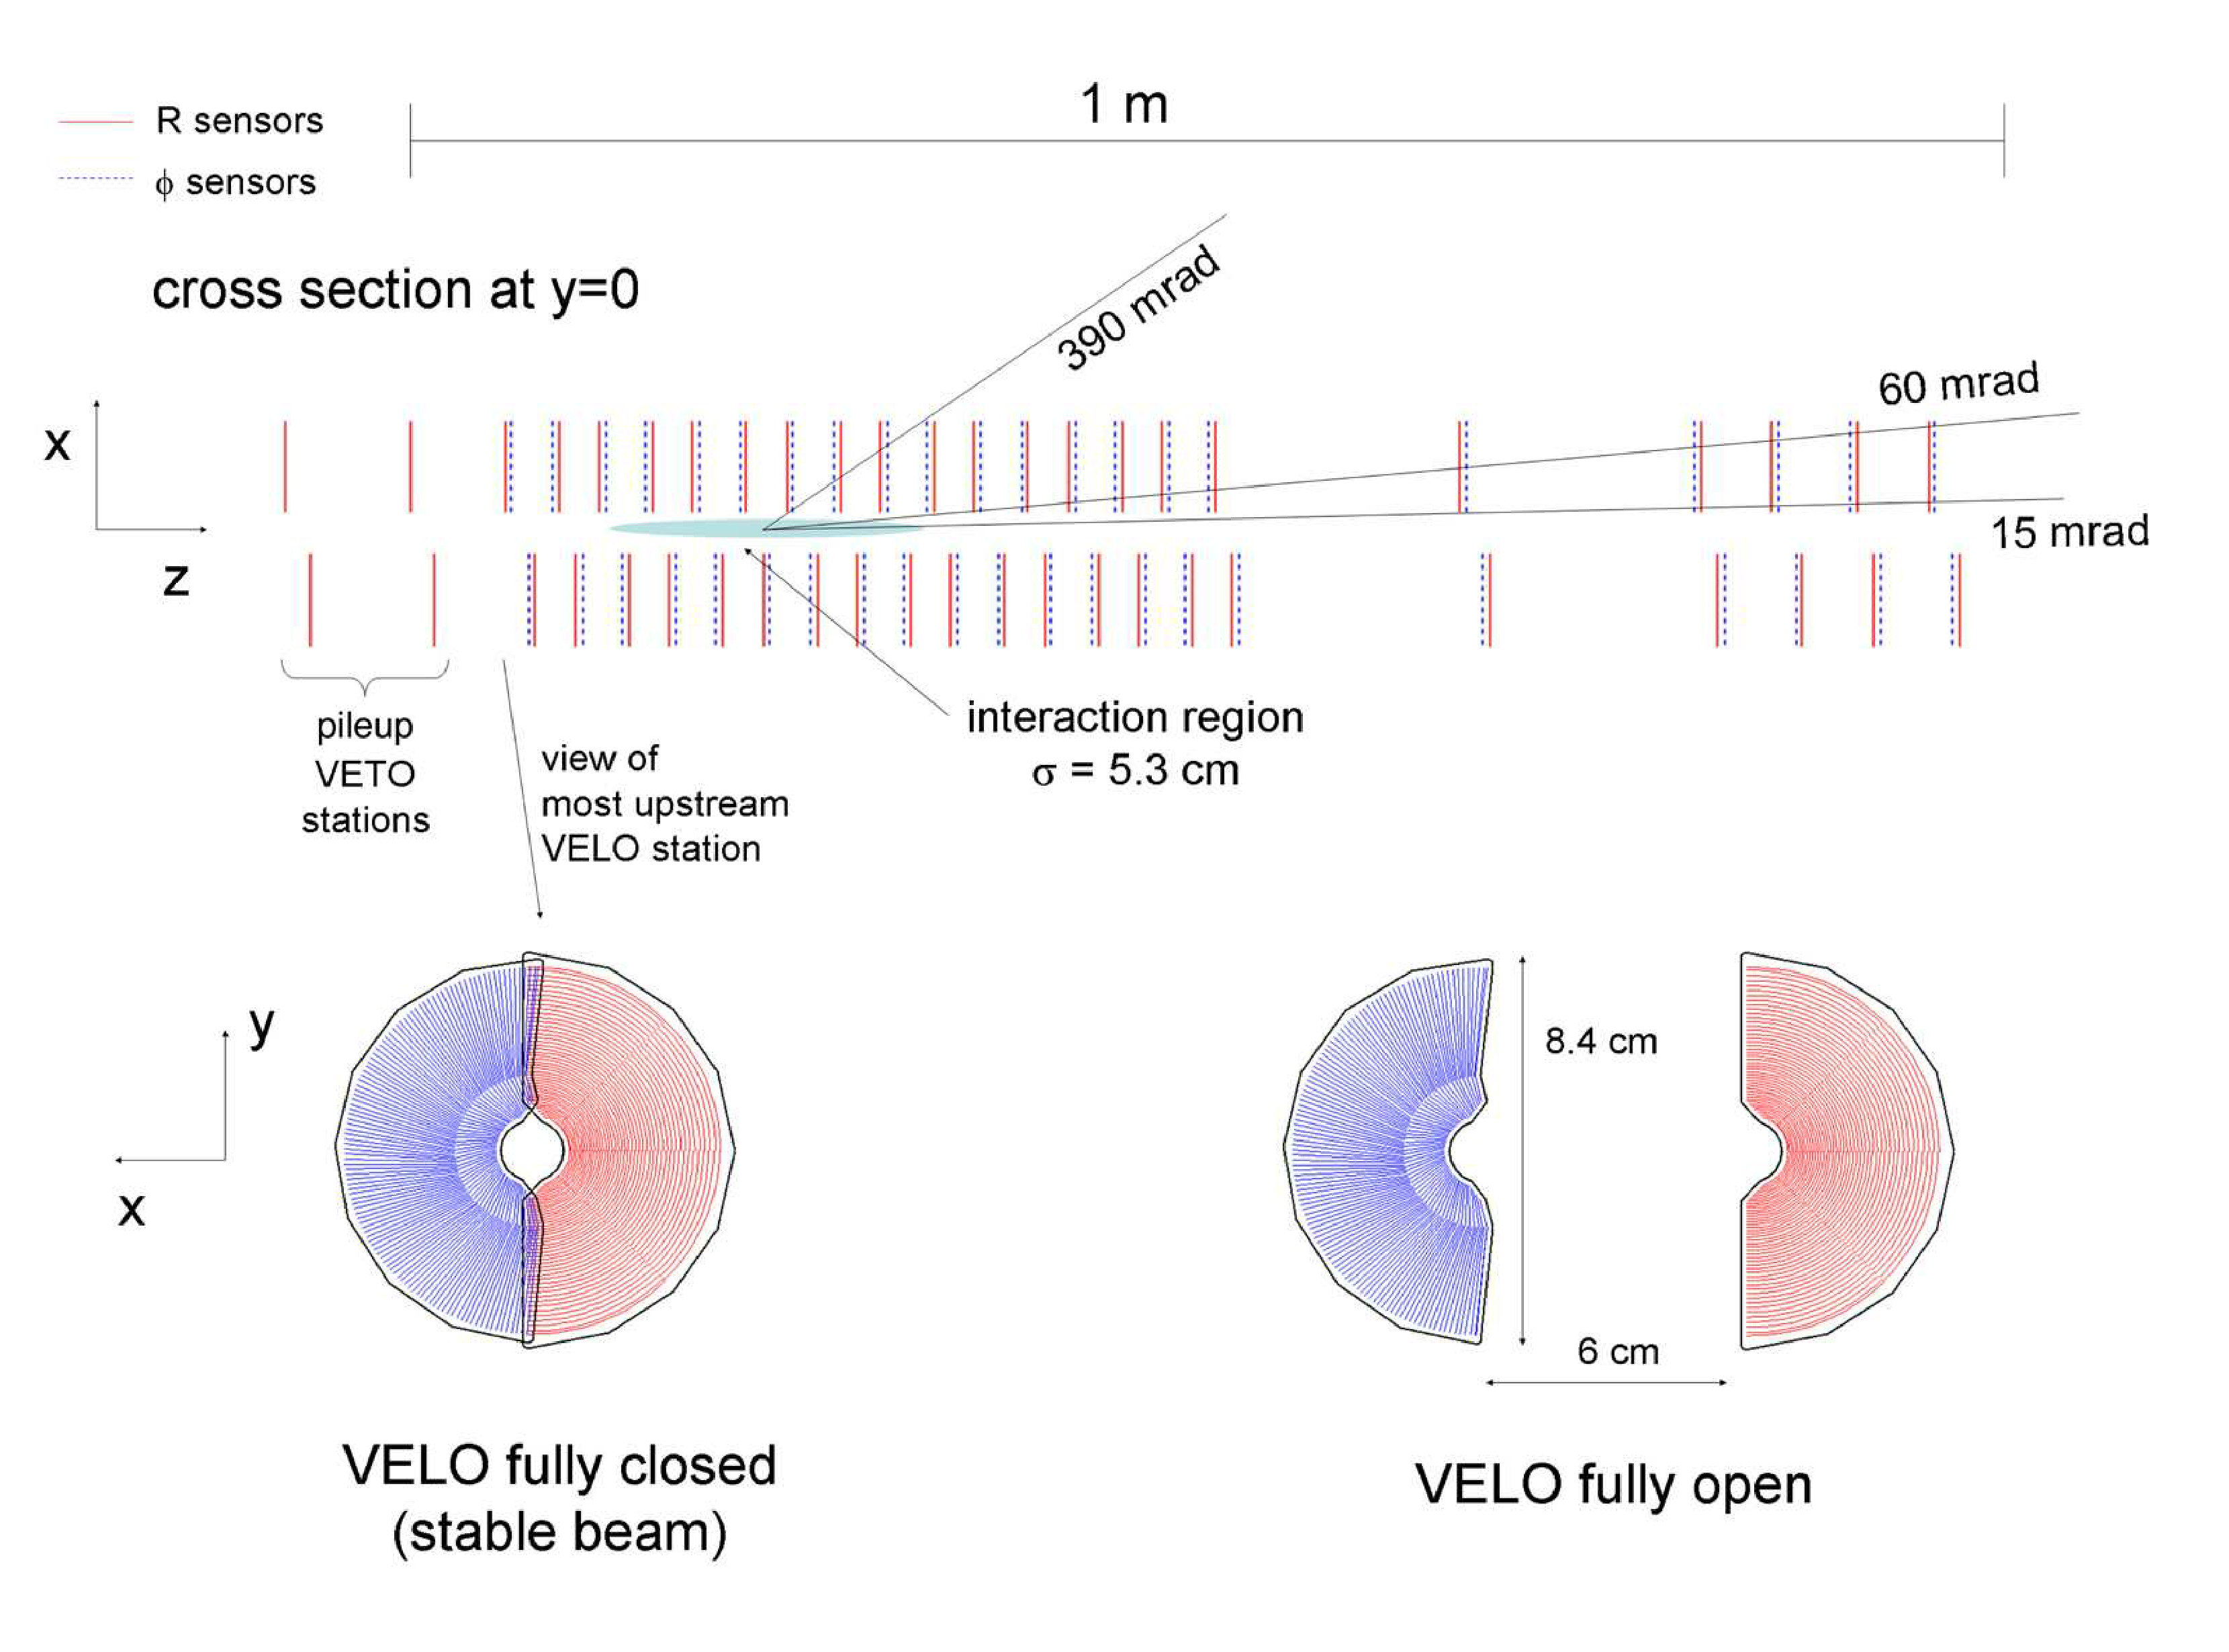
\includegraphics[width=0.8\textwidth]{velo}
  \end{center}
  \caption[Diagram of the LHCb Vertex Locator]
  {
    The layout of silicon sensors the \velo in showing $r$ sensors in red and $\phi$ sensors in
    blue.
    A cross section at $y=0$ in the \plane{x}{z} is shown while the \velo is closed.
    Along side these are slices in the \plane{x}{y}, with the \velo closed and open.
  }
  \label{fig:lhcb:velo}
\end{figure}

Hits recorded in the tracking system are fitted to tracks, and in order to decrease the
distance of extrapolation of tracks to vertices,
the active area of the \velo starts $8\mm$ from the beam line.
This is made possible because each module is split into two halves which are retracted when the
\lhc beam is being injected, and then closed when the beam is declared stable and data taking can
begin.
Its design leads to a detector with high impact parameter resolution, which can detect tracks
emerging from a $pp$ interaction located in the range $1.6<\eta<4.9$ and $|z|<10.6\cm$.
The geometry of the tracking stations is shown in \Fig{fig:lhcb:tracking}.

\begin{figure}
  \begin{center}
    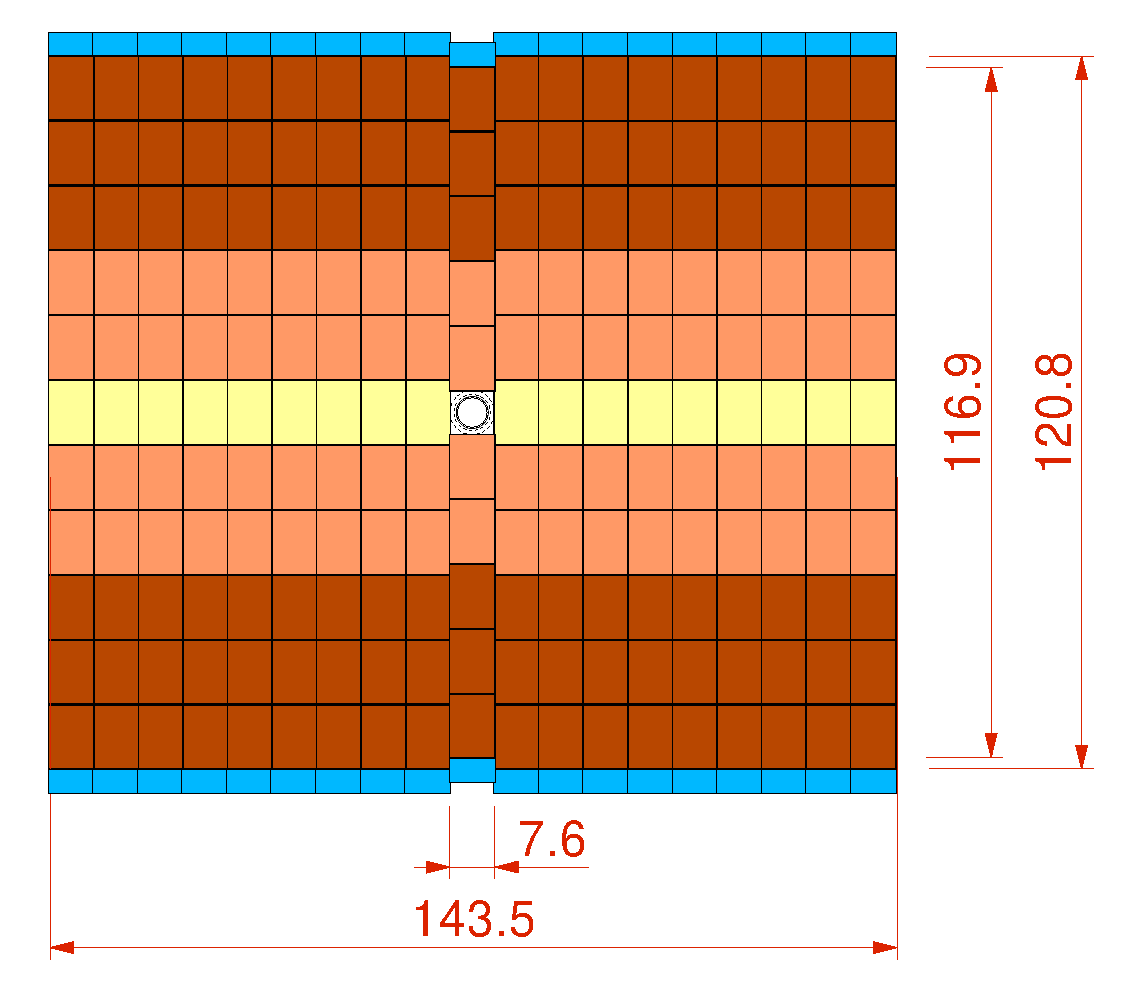
\includegraphics[width=0.5\textwidth]{TTfront}
    \caption[Diagram of the LHCb Tracker Turicensis]
    {
      Schematic diagram of a single stereo \ttracker layer oriented in the $x$-direction.
      Different colours indicate readout density.
      All units are in cm.
    }
    \label{fig:lhcb:tt}
  \end{center}
\end{figure}

Charged particles leaving the \velo are next observed traversing the \ttracker (assuming that they
remain within the \lhcb detector volume).
Immediately downstream of the \ttracker is the \lhcb magnet, followed by the remaining three
tracking stations (T1--3).
The T1--3 tracking stations are each made of two different technologies, the area nearest the beam,
aptly named the \intr, shares silicon sensor technology adopted by the \ttracker,
while the \ot uses a straw drift-tube technology.
Each tracking station exhibits an $x-u-v-x$ geometry, where $u$ and $v$ are rotated by $-5^\circ$ and
$+5^\circ$ with respect to the $y$-axis.

Together, the \ttracker and \intr are referred to as the \st.
The \st uses silicon strip sensors with a pitch of $200\mum$.
The \ttracker is the only part of the tracking system that is not used in the trigger, but is
instead used to improve the resolution in reconstructing tracks offline.
To do this, the \ttracker aids the extrapolation of tracks from T1--3, --- and the muon stations
--- to the \velo.
Spacial resolution of the \ttracker is increased by having a large gap, around $27\cm$, between
each stereo layer of the detector, whereas in the \intr the gap is about $4\cm$.
To cope with higher occupancy nearest the beam line, the \ttracker has a increased readout density
closer to $y=0$.
A schematic diagram of a \ttracker layer is shown in \Fig{fig:lhcb:tt}.

Figure~\ref{fig:lhcb:tracking} shows a diagram of T1--3.
The \intr{s} each occupy a small cross-shaped region, is closest to the beam in T1--3.
The \ot is constructed from modules each containing two staggered planes of densely packed straw
tubes, each with a diameter of  $4.9\mm$.
In all the \velo, \st and \ot give the \lhcb detector excellent momentum resolution;
$\tfrac{\Delta p}{p}$ between 0.4 and 0.6\,\% for particles with momenta of $5\gev$ and $100\gev$
respectively.
%Essential for good resolution of the B invariant mass.

\begin{figure}
  \begin{center}
    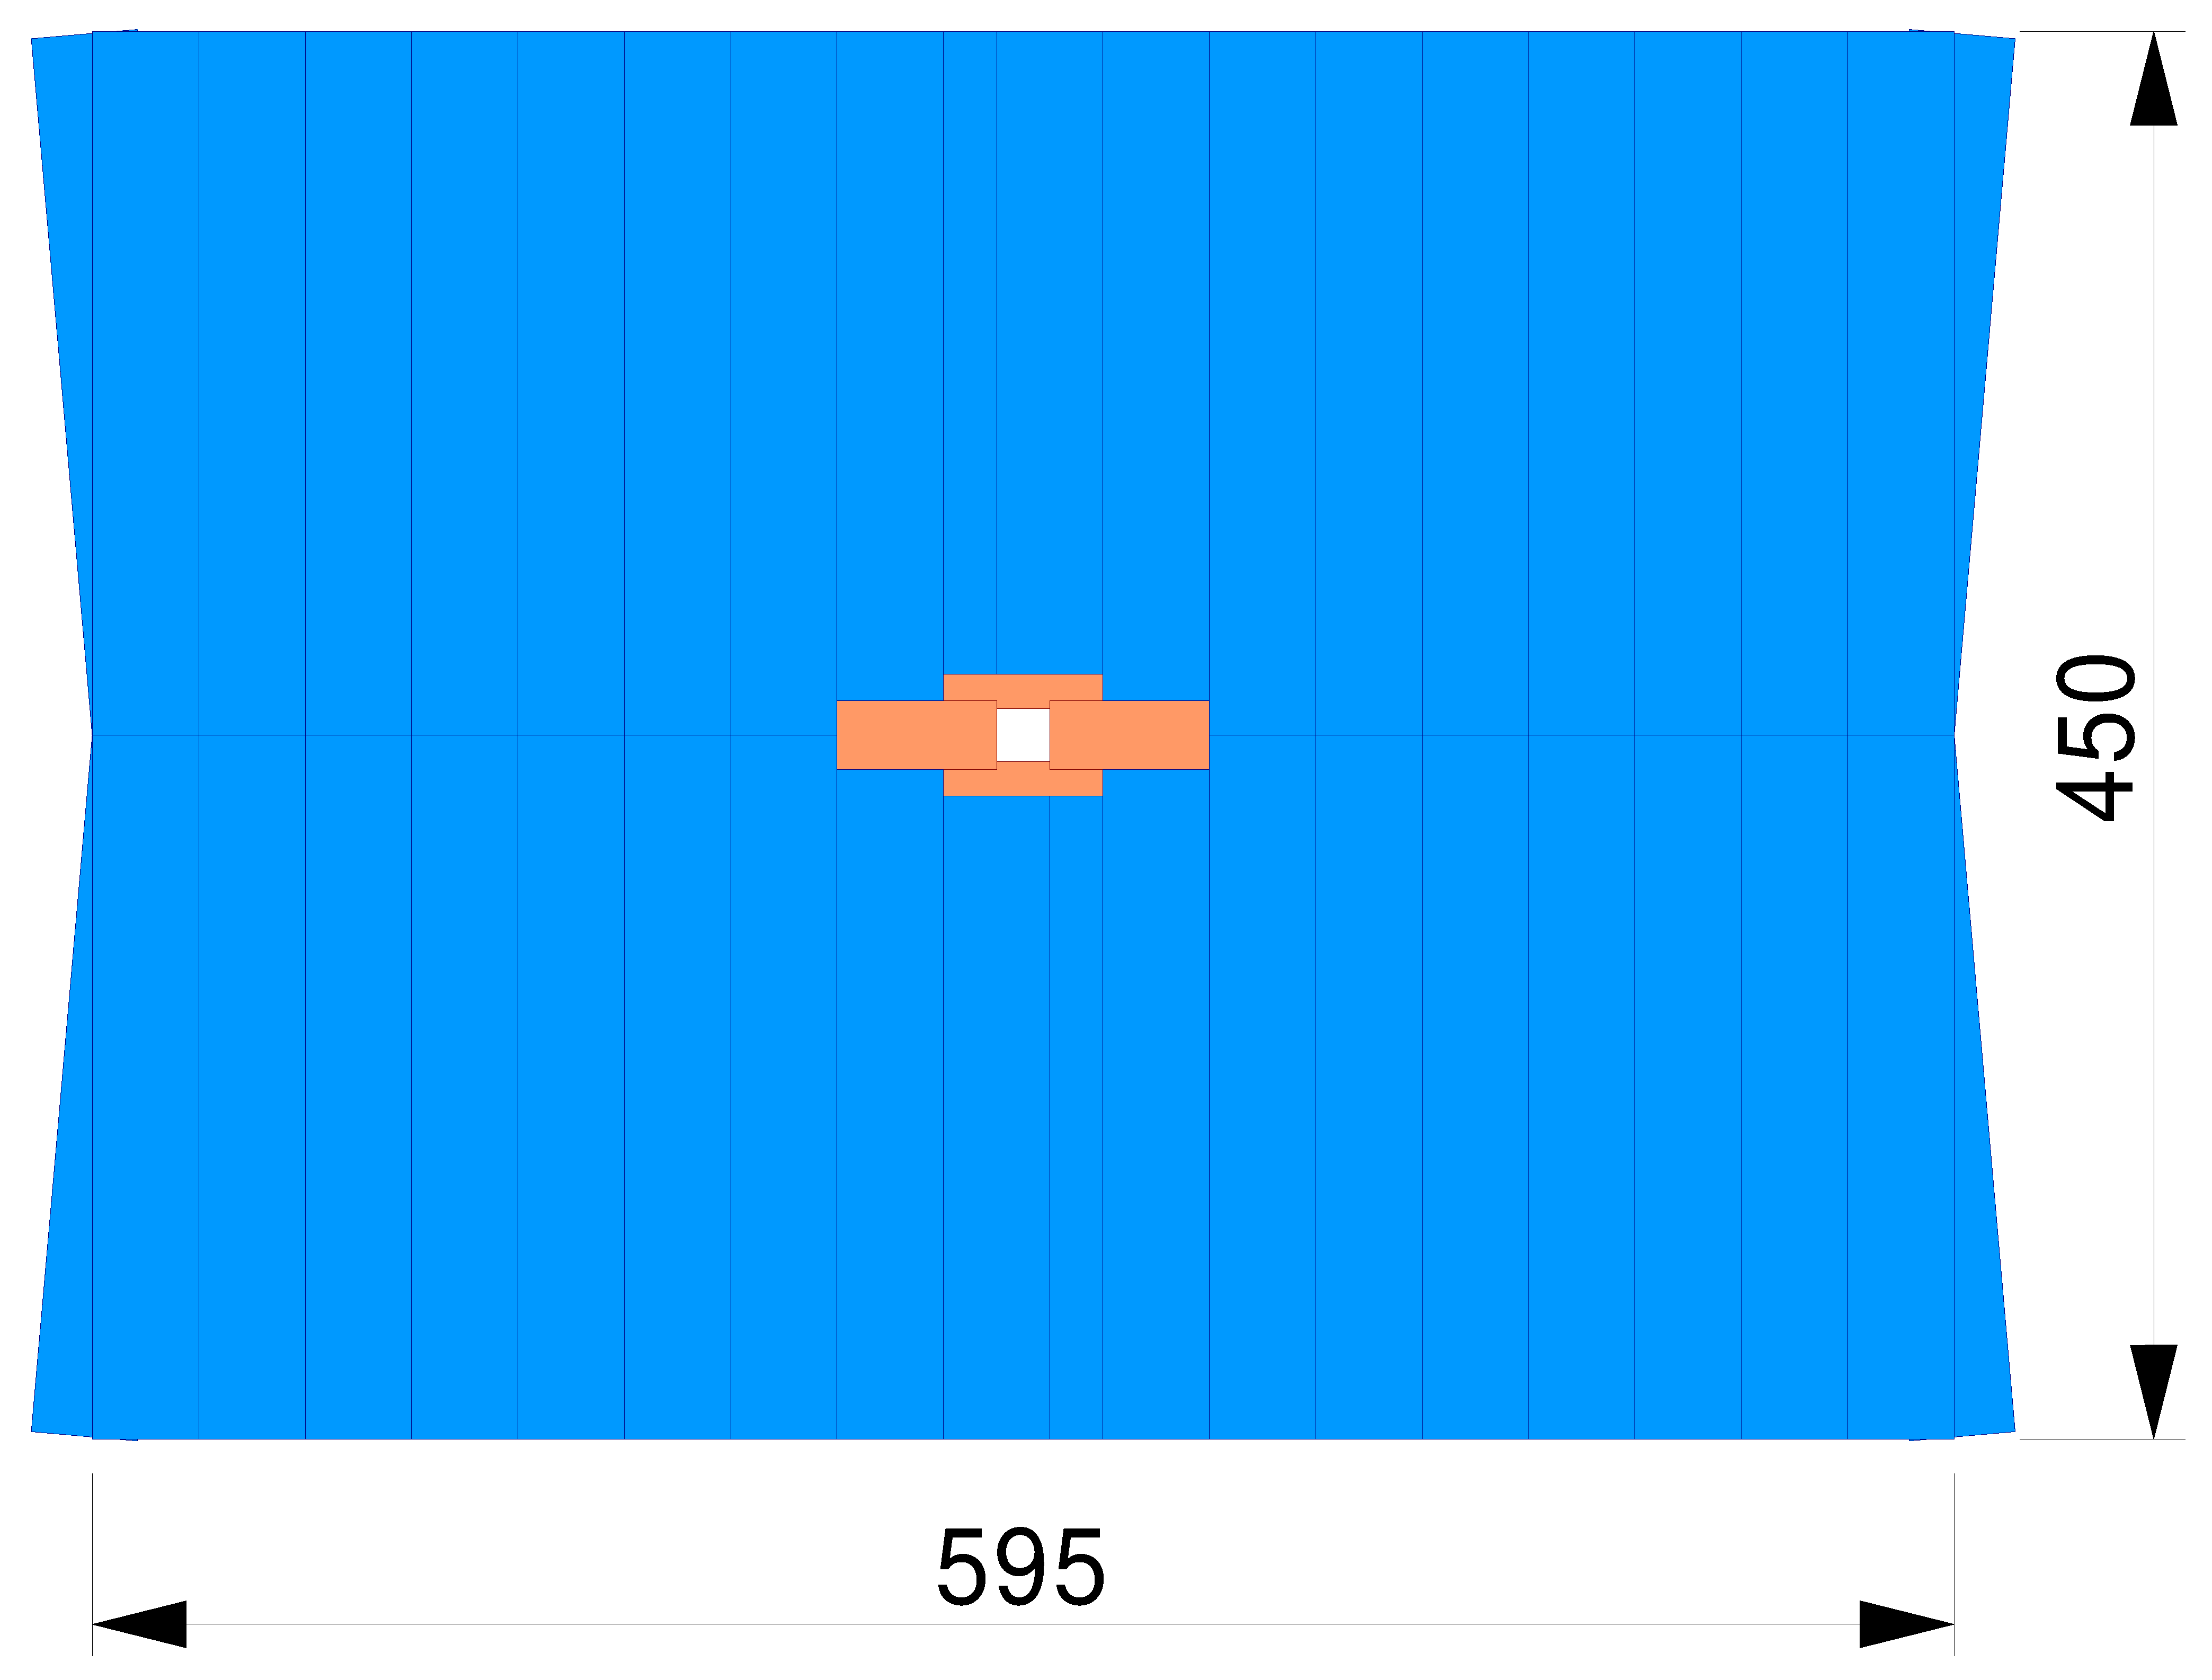
\includegraphics[height=0.18\textheight]{stfront}
    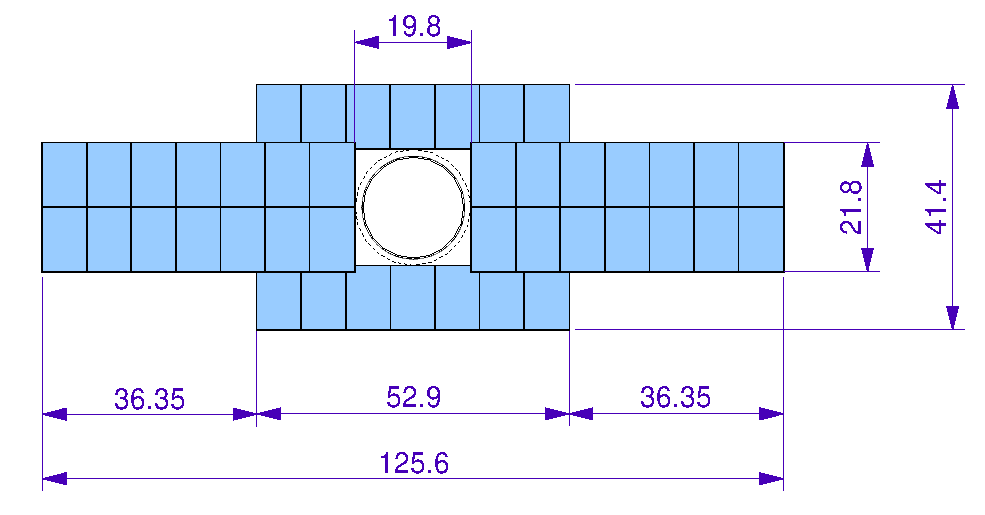
\includegraphics[height=0.19\textheight]{st2}
  \end{center}
  \caption[Diagram of the LHCb tracking stations T1--3]
  {
      Schematic diagram of the (left) tracking stations T1--3, where the outer region is the \ot,
      and the inner cross is the silicon \intr.
      A zoom of an $x$ oriented \intr layer is also shown (right).
      All units are in cm.
  }
  \label{fig:lhcb:tracking}
\end{figure}



